\documentclass[a4paper,12pt]{article}
\usepackage[margin=1in]{geometry} % Set 1-inch margins
\usepackage{graphicx}

\title{Practical Work 2: RPC File Transfer}
\author{}
\date{}

\begin{document}

\maketitle

\section*{1. RPC Service Design}
The RPC (Remote Procedure Call) service is designed as follows:
\begin{enumerate}
    \item The system uses XML-RPC as the communication protocol between the client and server.
    \item The server exposes three main remote functions:
    \begin{itemize}
        \item \texttt{upload\_file(filename, file\_data)}: Accepts a file from the client and saves it on the server.
        \item \texttt{download\_file(filename)}: Sends a file from the server to the client.
        \item \texttt{exit\_server()}: Gracefully terminates the server.
    \end{itemize}
    \item The client uses these remote functions to perform file transfers and communicate with the server.
\end{enumerate}


\section*{2. System Organization}
The system is organized into the following components:
\begin{enumerate}
    \item \textbf{Client:}
    \begin{itemize}
        \item Connects to the RPC server using XML-RPC.
        \item Sends commands such as \texttt{upload}, \texttt{download}, and \texttt{exit}.
        \item Handles file reading and writing on the client side.
    \end{itemize}
    \item \textbf{Server:}
    \begin{itemize}
        \item Provides remote procedures to handle client requests.
        \item Manages files (saves uploaded files, sends files for download).
        \item Terminates upon receiving the \texttt{exit} command.
    \end{itemize}
\end{enumerate}

\noindent \textbf{Figure: System Organization Diagram}
\begin{figure}[h!]
    \centering
    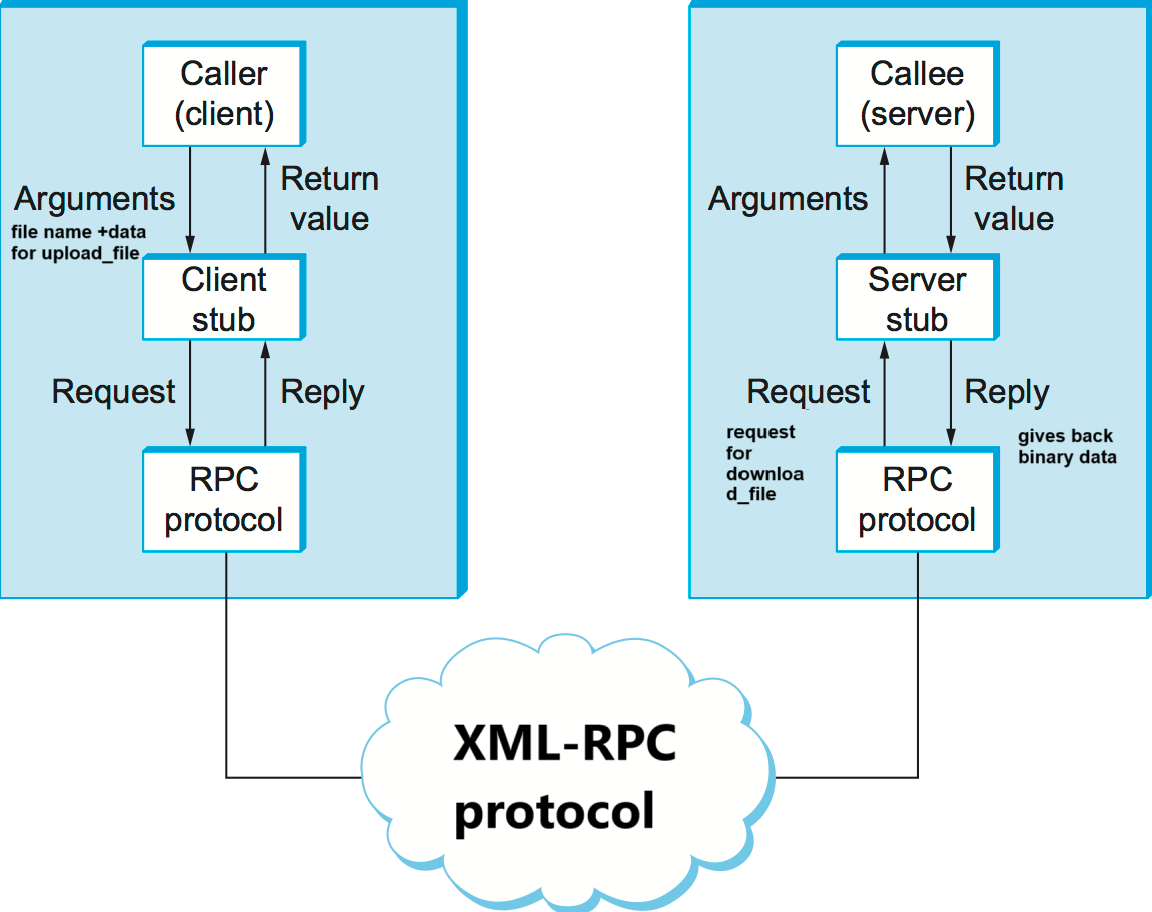
\includegraphics[width=0.8\textwidth]{design.png} 
    \caption{System Architecture}
\end{figure}

\section*{3. Implementation of File Transfer}
The file transfer is implemented using the following key steps:
\begin{enumerate}
    \item \textbf{File Upload:}
    \begin{itemize}
        \item The client reads the file, encodes it into binary, and sends it to the server using the \texttt{upload\_file()} function.
        \item The server receives the binary data and writes it to a file on the server disk.
    \end{itemize}
    \item \textbf{File Download:}
    \begin{itemize}
        \item The client requests a file using the \texttt{download\_file()} function.
        \item The server reads the file, encodes it into binary, and sends it back to the client.
    \end{itemize}
    \item \textbf{Server Termination:}
    \begin{itemize}
        \item The client sends an \texttt{exit} command using the \texttt{exit\_server()} function.
        \item The server terminates gracefully after processing the command.
    \end{itemize}
\end{enumerate}


\section*{4. Team Contributions}
The tasks were distributed as follows among the five team members:
\begin{itemize}
    \item \textbf{Research on XML-RPC Technology:} Do Thi Huong Tra (BA12-174) and Vu Hoang Mai Nhi (22BI13352)
    \item \textbf{Design of the RPC Service and API:} Cao Nhat Nam (22BI13320) 
    \item \textbf{Implementation of File Upload Functionality,File Download and Exit Functionality:}Pham Ngoc Minh Chau (22BI13063)
    \item \textbf{Testing and Report Writing:} Bui Nguyen Ngoc Huyen (22BI13199)
\end{itemize}

\end{document}
